{% -*- mode: LaTeX; TeX-PDF-mode: t; TeX-master: "manual"; -*-
}


\chapter{An Overview of the \ei Framework}
\label{ch:overview}

The \ei framework provides a simple way to build interfaces, e.g, a
web-interface or an Eclipse plug-in, for tools written in (almost) any
programming language.
%
Moreover, it does not require the programmer to be familiar with any
GUI library or web programming. Roughly, the only requirement is that
the application can be executed from a command-line and that its
output goes to the standard output.
%
With the \ei framework we achieve the goal: \emph{build an application
  once, and get several sophisticated interfaces for free}.
%
In the rest of this chapter we explain the different components of
this framework, and how they are combined to achieve the above goal.
%
As will bed noticed later, the \ei framework was developed with
program analysis tools in mind, this why the graphical user interfaces
that it provides are basically developing environment that allow
editing programs, etc.

\section{The Architecture of \ei}
\label{ch:overview:arch}

\begin{figure}[h]
\begin{center}
\fbox{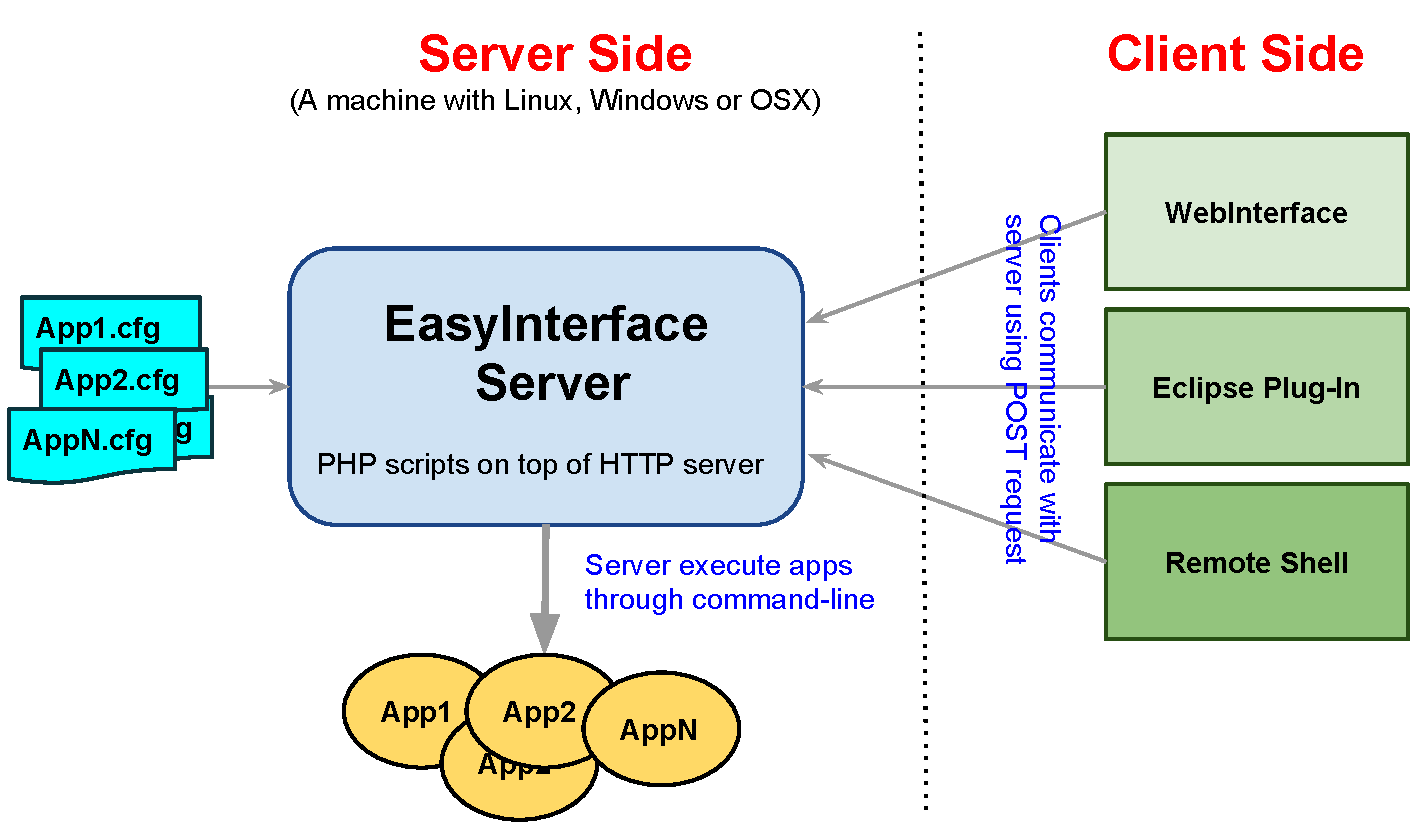
\includegraphics[width=0.5\textwidth]{fig/ei.pdf}}
\end{center}
\caption{The Architecture of the \ei Framework}
\label{fig:eiframework}
\end{figure}

The architecture of the \ei framework is depicted in
Figure~\ref{fig:eiframework}. It includes two main components:
%
(1) \emph{server side}: a machine with several applications (the
circles \texttt{App1}, \texttt{App2}, etc.) that can be executed from
a command-line and produce their output to the standard output. These
are the applications that we want to make available for the outside
world, i.e., execute them as services on the internet; and
%
(2) \emph{client side}: several clients that makes it easy to
  communicate with the server side to execute application, etc.
%
In what follows we start explaining the inner components of the server
side, and which problems they solve, and then we move on to explain the
client side.

\subsection{The Server Side}
\label{ch:overview:arch:server}

The problem that we want to solve at the server side is: 
%
\begin{quote}
  provide a uniform way for accessing the locally installed
  application as services (i.e., through the internet).
\end{quote}
%
This problem is solved by the \ei server, which is collection of PHP
programs that run on an HTTP server. The \ei server allows specifying
how a local applications can be executed and which parameter they take
using simple configuration files (\texttt{App1.cfg},
\texttt{App2.cfg}, etc.). For example, the following is a snippet of
such configuration file:

\medskip
\begin{lstlisting}
<app id='myapp' visible="true">
  ...
  <execinfo method="cmdline">
    <cmdlineapp>./default/myapp.sh _ei_parameters</cmdlineapp>
  </execinfo>
  <parameters prefix = "-" check="false">
    ...
    <selectone name="c">
      <option value="1" />
      <option value="2" />
    </selectone>
  </parameters>
</app>
\end{lstlisting}

\medskip
\noindent
This XML defines an application that has a unique identifier
\lst{myapp}.  The \lst{cmdlineapp} tag is a template that describes
how to execute the application from a command-line. Here
\lst{_ei_parameters} is a template parameter that will be replaced by
an appropriate value. The \lst{parameters} tag includes a list of
parameters accepted by the application. For example, there is a
parameter called ``\texttt{c}'' that can take one of the values $1$ or
$2$.
%
Once the configuration file is installed on the \ei server, anyone can
access the application using an HTTP POST request that include
something similar to the following:

\medskip
\begin{lstlisting}
{
  (*command: "execute",*)
  (*app\_id: "myapp",*)
  (*parameters:*) {
     (*c: ["1"],*)
     (*...*)
  },
  (*...*)
}
\end{lstlisting} 

\medskip
\noindent
When the \ei server receives such a request, it generates a
corresponding command-line (according to what is describe din the
configuration file), executes it, and redirect the standard output
back to the client.

\section{The Clients Side}
\label{ch:overview:arch:clients}

Although now we have a relatively easy way to execute application on
the server side, we still need to make HTTP POST requests, etc. We are
interesting replacing this by (graphical) user interfaces that does so
automatically. For this, we provide clients that allow the user to
select an application to execute, set the values of the corresponding
parameters and then it automatically generate the corresponding
request and communicate with the \ei server.

The first client is a web-interface that can be executed in a browser
and looks like an environment for developing programs, the second is
an Eclipse-plugin that runs inside the Eclipse IDE, and the last we
call a remote-shell that can be used from a command-line.
%
Now since the web-client and the Eclipse plugin include a developing
environment, it would be nice to provide away such that apps can view
their output in a graphical way (e.g., open dialog box, highlight code
lines, add markers in the editor). For this, the \ei framework defines
a text-based output language that can be used by the applications to
describe their output, and the clients include an interpreter that
transform this text-based command into graphical element.








%%% Local Variables: 
%%% mode: latex
%%% TeX-master: "manual"
%%% End: 
